\newcommand\runit{{\hat{\bm{r}}}}
\newcommand\thetaunit{{\hat{\bm{\theta}}}}
\newcommand\phiunit{{\hat{\bm{\phi}}}}

\chapter{{\it \'Etude}: on magnetic reconnection in 3D magnetospheres of pulsars}

\label{ch:pulsar}

In $\gamma$-ray pulsars a significant fraction of the spin-down power (few to ten percent) is converted into high energy photons \citep{2013ApJS..208...17A}. This suggests that somewhere in the magnetosphere the Poynting flux radiated by the rotating star is efficiently converted into plasma kinetic energy and, ultimately, $\gamma$-rays. Magnetic reconnection in the equatorial current sheet is a likely candidate to power this energy extraction. The emergence of the current sheet in plasma-filled magnetospheres of neutron stars has been predicted in force-free formulation \citep{1999ApJ...511..351C, 2006ApJ...648L..51S}, while kinetic plasma simulations allowed to model them self-consistently, capturing the process of magnetic reconnection \citep{2014ApJ...785L..33P,2014ApJ...795L..22C,2015MNRAS.448..606C,2015MNRAS.449.2759B,2020A&A...642A.204C}. 2D simulations of axisymmetric magnetospheres were able to achieve significant separation of scales between the macroscopic extent of the current layer and the microscopic plasma-kinetic scale. This is critical for simulations of tearing unstable current sheets and magnetic reconnection to properly capture the hierarchical chain of magnetic islands (plasmoids) extending from the microscopic scales to the size of the whole system. However, the dynamics of a 2D reconnecting current sheet may be different from that in 3D. Current layers in 3D are prone to other kinetic instabilities, such as the kink instability, that additionally disrupt the layer on top of the tearing instability, which may lead to inhibited dissipation rate \citep{2021arXiv210500009Z,2020arXiv200802743G,2021arXiv210602790W}. On top of that, neutron stars which have magnetic axes misaligned with respect to their rotation axes have intrinsically non-axisymmetric magnetospheres and, as a result, more complex structures of current layers. 3D simulations are, thus, required to properly study both the onset and the dynamics of the magnetospheric current layer.

While 3D simulations properly recreate the general structure of the magnetosphere, the complex dynamics of the current layer is still largely unstudied due to rather limited scale separation. In this work we make an attempt to properly capture the microphysics of the current sheet in 3D PIC simulations by extending the separation of macro-to-micro scales to $\gtrsim 100$. We achieve this by employing a hybrid approach for particle pushing in our simulations described by \cite{2020ApJS..251...10B}. We also include a self-consistent synchrotron radiation reaction force. By properly modeling this radiative reconnection dynamics in the current sheet, we study how particles are accelerated in this process, and examine the key parameters that affect the amount of dissipated energy and the emerging $\gamma$-ray spectra.

We begin in section~\ref{sec:psr-magnetosphere} with a brief introduction to the 3D structure of the magnetosphere, and the numerical setup we employ to produce this solution. We then describe the energy dissipation process in the magnetically reconnecting current layer and demonstrate that the rate of the reconnection set by plasma microphysics controls the overall dissipation rate in the magnetosphere (section~\ref{sec:psr-dissipation}). We conclude with section~\ref{sec:psr-radiation} where we study the particle acceleration process mediated by a synchrotron radiation reaction. We show how the interplay between radiative losses and acceleration in magnetic reconnection explains the observed diversity of $\gamma$-ray spectra in pulsars. 

\section{Plasma-filled pulsar magnetospheres} 
\label{sec:psr-magnetosphere}
Pair-producing cascade near the neutron star surface has long been thought to populate the neutron star magnetospheres with pair-plasma \citep{1969ApJ...157..869G, 1975ApJ...196...51R}. For the most energetic young pulsars this pair-producing cascade is highly efficient \citep{2015ApJ...810..144T, 2019ApJ...871...12T}. Their magnetospheres are quenched with enough plasma to effectively screen large-scale accelerating electric fields, localizing and constraining the regions with $\bm{E}\cdot\bm{B} \ne 0$ to microscopic scales. Currents induced by the motion of this plasma also modify the large-scale structure of the magnetic fields. As a result, the global structure of young neutron star magnetospheres is well described by the so-called force-free (or plasma-filled) solution.

Charge density necessary to sustain this force-free solution is called \emph{Goldreich-Julian} (GJ) density,

\begin{equation}
    \rho_{\rm GJ} = \frac{\bm{\Omega} \cdot\bm{B}}{2\pi c}.
\end{equation}
\noindent That is, if enough plasma is provided, the local steady-state charge density that will be established to screen the accelerating electric field is $\rho_{\rm GJ}$. Magnetospheres that do not have enough plasma supply to screen parallel electric fields may have somewhat different structures; however, they are beyond the scope of this work \citep[see, e.g.,][]{2020ApJ...889...69C}.

According to force-free solution the plasma close to the surface corotates with the neutron star, flowing along almost poloidal magnetic field lines that start and end at the surface of the star. This corotation continues for distances from the rotation axis less than $R_{\rm LC}=c/\Omega$ ($\Omega$ being the rotation frequency of the neutron star), the \emph{light cylinder}. From that point the plasma can no longer corotate with the star, and the bulk of the particles flies away from the star almost radially, forming the so-called \emph{pulsar wind}.

\begin{figure}[htb]
\centering
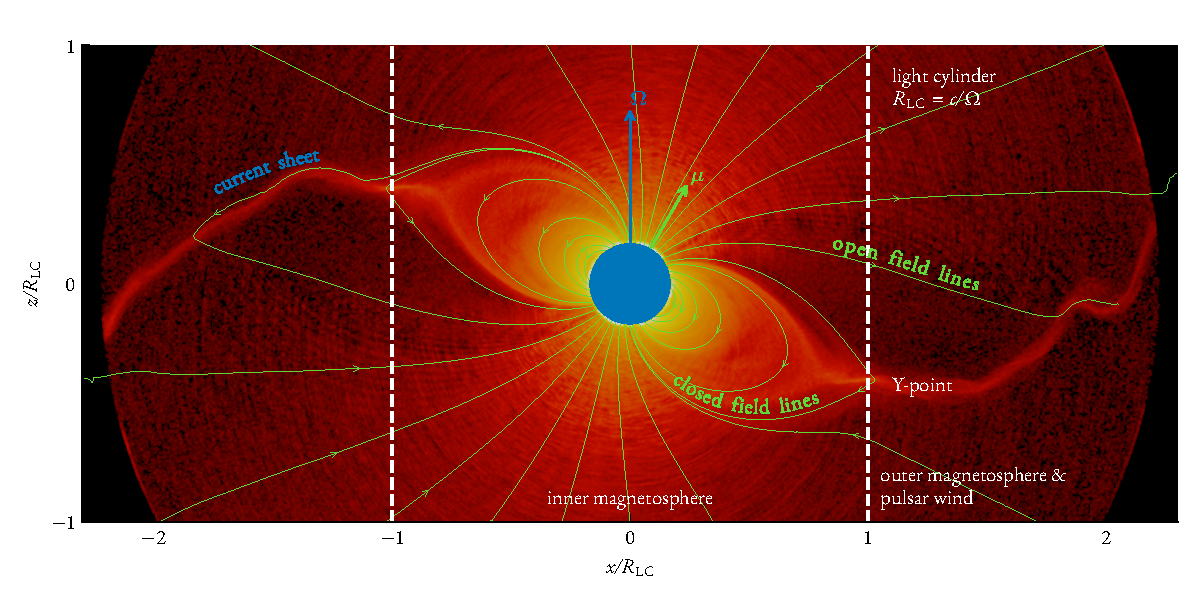
\includegraphics[width=\columnwidth]{figures/ch3-pulsar/fig1.pdf}
\caption{Poloidal slice of the 3D plasma density from a simulation of an inclined rotator with $\chi=20^\circ$. The surface of the neutron star and the direction of its rotation are shown in blue. Magnetic field lines traced from the surface of the star, as well as the direction of the magnetic moment, are shown in green. The light cylinder, $R_{\rm LC}$, shown with white dashed lines, separates the inner magnetosphere from the outer magnetosphere and the wind. Current sheet originating near the Y-point and spreading to the outer magnetosphere is clearly visible. }
\label{fig:psr-pulsardraft}
\end{figure}

Schematically this solution is demonstrated in Figure~\ref{fig:psr-pulsardraft}. While in the inner magnetosphere (inside the light cylinder) magnetic field lines are almost purely poloidal, in the outer magnetosphere they have also a toroidal component. Opposing field lines from the northern and southern hemispheres of the neutron star are divided in the outer magnetosphere by a \emph{current sheet}. The physics of this current sheet is the main topic of the current work. 

The thickness of this current sheet is microscopic. Its characteristic scale does not exceed few-to-tens of plasma skin depths, $d_e$:
\begin{equation}
    d_e = c/\omega_{{\rm p}e},
\end{equation}
\noindent where $\omega_{{\rm p}e}$ is the plasma frequency for relativistic electron-positron pairs in the current sheet. For the Crab pulsar this parameter close to the light cylinder is of the order of a few centimeters, assuming the number density in the current sheet is $\sim 10^4|\rho_{\rm GJ}/e|$ \citep{1996A&A...311..172L}. The light cylinder, on the other hand, is almost $8$ orders of magnitude larger (for Crab it is $\sim 1500$ kilometers). Nevertheless, the dynamics of this microscopically thin current sheet is of critical importance. In this region the magnetic energy dissipation takes place that powers particle acceleration and the observed high-energy emission from pulsars.

\subsection*{\small\it Numerical setup}

Kinetic plasma simulations are necessary to properly capture the plasma processes in the magnetospheric current sheet and the energy dissipation process. In this work we employ particle-in-cell (PIC) algorithm implemented in the \texttt{Tristan-MP v2} code designed by \cite{tristanv2} to simulate the 3D dynamics of the entire magnetosphere. Our simulations start with an empty Cartesian domain of the size $\sim 5 R_{\rm LC}$ and a perfectly conducting rotating sphere in the center. Dipolar magnetic field is imposed as a boundary condition near the surface of the sphere; near outer boundaries the fields are damped to zero and the particles are free to outflow. It is important to note here, that in reality the magnetic field structure at the surface of the neutron star is not necessarily dipolar \citep{2019ApJ...887L..23B}. The reason we allow for this simplification is that the structure of the magnetosphere at distances $R_*\ll r\sim R_{\rm LC}$ ($R_*$ being the stellar radius) is mostly dictated by the dipolar component, that decays slowest with the distance \citep{2020ApJ...893L..38C}. 

To fill the magnetosphere with plasma we mimic the pair-production process near the surface of the star by injecting pair-plasma at a rate proportional to the local GJ density: $\dot{n}(\theta,\phi) = f_{\rm inj}|\rho_{\rm GJ}(\theta,\phi) / e|$. $f_{\rm inj}$ is a dimensionless number which we typically set to $1$; it controls the injection multiplicity. The exact value of this number is unimportant, as long as enough plasma is injected to establish the force-free solution. We also give a marginal initial velocity to the newly injected particles along the local magnetic field lines  (typically a Lorentz factor of $\gamma\approx 2$) \citep[similar technique has been previously used by][]{2015MNRAS.448..606C, 2015MNRAS.449.2759B}. After a brief transient lasting for about $1$ rotation period of the star, $P$, steady-state solution is established (see Figure~\ref{fig:psr-pulsardraft}) which closely resembles the force-free solution. Deviations from the force-free solution are at the scale of the local plasma skin-depth, $d_{e}$. 

To be able to properly resolve the skin depth almost everywhere with at least a few simulation cells (with the exception of the surface of the star) we greatly exaggerate the scale separation compared to realistic pulsars. First of all, in a series of our simulations the radius of the star is resolved by $75$ cells (we will denote $\Delta x$ as the size of the cell), while the period is $6200$ timesteps (we will denote $\Delta t$ as the length of a timestep). By having the speed of light $c=0.45\Delta x/\Delta t$,\footnote{This is the maximum we can allow to still satisfy the Courant–Friedrichs–Lewy (CFL) condition.} this makes the light cylinder about $R_{\rm LC}\sim 440\Delta x$, or $\sim 6$ times the radius of the star. For most of the astrophysical pulsars this ratio, $R_{\rm LC}/R_*$, is greater than $100$ (in particular, for Crab pulsar this value is about $150$), while only for the fastest spinning millisecond ones this value can be close to few tens. The downscaled ratio of $R_{\rm LC}/R_*$ in our simulations, however, only marginally affects the global structure of the magnetosphere, especially outside the light cylinder. 

More important assumption we make, is that we resolve the plasma skin depth near the light cylinder with at least a few cells: $d_e\sim \text{few}~\Delta x$. This means that the scale separation between macroscopic and microscopic (plasma kinetic) length scales is at most $\sim200$ in our highest resolution simulation (c.f. with almost $8$ orders of magnitude scale separation in realistic pulsars). Large scale separation ensures that the growth of microscopic plasma instabilities, that develop at kinetic timescales, $\omega_{{\rm p}e}^{-1}$, is much faster than the dynamical timescale characterized by rotation period, $P$. Localized 2D simulations \citep[see, e.g.,][]{2016ApJ...816L...8W} show that at scale separation $\gtrsim 100$ kinetic instabilities establish an asymptotic regime, which justifies our choice of $R_{\rm LC} / d_e^{\rm LC} \sim \omega_{{\rm p}e}^{\rm LC}/\Omega \sim 200$. 
% More details on these assumptions are discussed in the Appendix \ref{sec:psr-appendixA}. 

Such a long timestep, $\Delta t$, and scale separation are only accessible because we employ a coupled guiding-center/Boris algorithm for solving particle equations of motion \citep{2020ApJS..251...10B}. This approach allows to ignore gyrations of most of the particles in the magnetosphere, reducing their motion to that of their guiding centers, while still recovering the ``proper'' equation of motion for high-energy particles in regions with vanishing magnetic field (i.e., current sheet).

Overall, there are three dimensionless parameters that we can vary independently in our simulations (apart from the obliquity angle, $\chi$):
\begin{itemize}
    \item $R_{\rm LC} / d_e^{\rm LC}$: the ratio of the size of the light cylinder and the plasma skin depth at a corresponding GJ plasma density, we refer to this as the scale separation of our simulation;
    \item $R_* / \Delta x$: the number of simulations cells per stellar radius, which we call the resolution of our simulation;
    \item $R_{\rm LC} / R_*$: the size of the light cylinder w.r.t. the size of the star.
\end{itemize}
\noindent In our simulations typical plasma densities do not exceed the local GJ plasma density by more than a few times, meaning that the skin-depth computed for a local GJ density, $d_e(n=n_{\rm GJ})$, is a good proxy for the actual skin-depth. All the other parameters are directly related to these three numbers.\footnote{In principle, $f_{\rm inj}$ is another free parameter that we can vary, but we keep it close to $1$, as values less than that are unable to fill the magnetosphere with enough plasma, while values much greater than $1$ are unable to properly screen the accelerating electric at the surface producing too much numerical noise.}
% (more details on that can be found in \ref{sec:psr-appendixA})

\begin{figure}[htb]
\centering
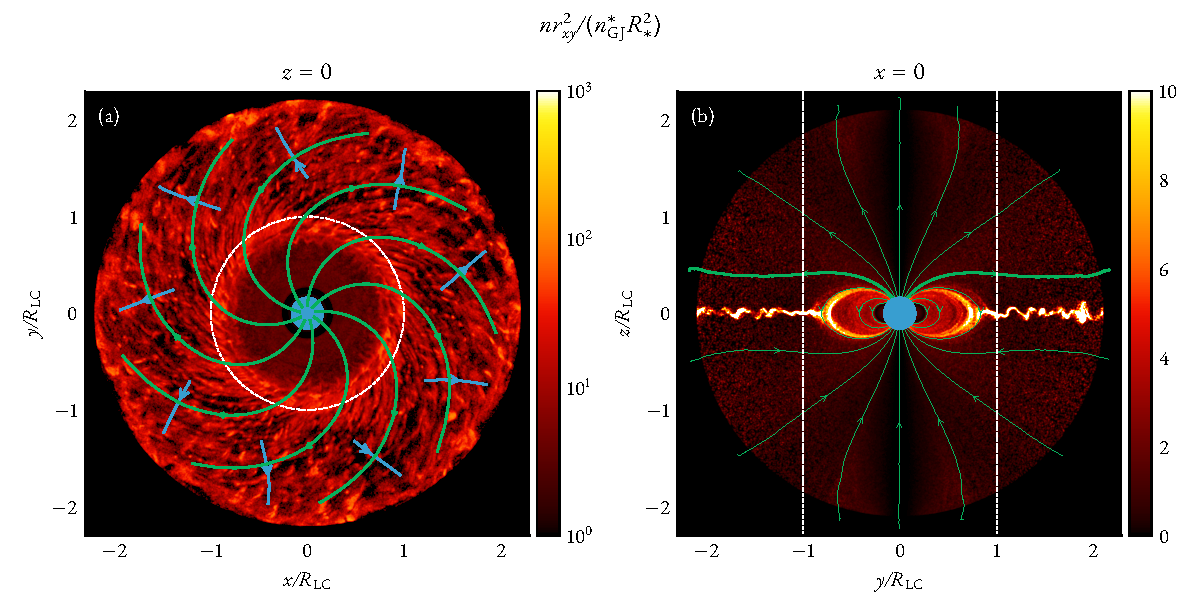
\includegraphics[width=\columnwidth]{figures/ch3-pulsar/fig2.pdf}
\caption{(a): equatorial slice of the plasma density from a simulation of an aligned rotator (\texttt{R75\_ang0}). Magnetic field lines originating at the stellar surface at about $30^\circ$ from the pole are shown with green lines. Blue arrows trace the direction of the equatorial current in the current sheet. White dashed circle indicates the light cylinder. Ripples in density are caused by the combined effect of two instabilities (tearing and kink) on the current sheet. (b): poloidal slice of the plasma from an axisymmetric simulation. As in (a), green lines show the direction of the magnetic field, while the two bold field lines correspond to the ones in panel (a). White dashed lines correspond to the position of the light cylinder. In this slice the kink-instability of the current sheet is apparent.}
\label{fig:psr-pulsarslice}
\end{figure}

\subsection*{\small\it Kinetic solution}
\label{psr:sub_kinetic_sol}

Let us closely inspect the structure of the magnetosphere in one of our simulations. For simplicity, we will consider an aligned rotator, $\chi=0^\circ$, where $R_{\rm LC} / d_e^{\rm LC} = 100$, $R_* = 75\Delta x$, and $R_{\rm LC} / R_* = 6$ (here and further we will refer to this simulation as \texttt{R75\_ang0}).\footnote{Simulations with the same basic parameters and other obliquity angles are, correspondingly, \texttt{R75\_ang20}, \texttt{R75\_ang60}, and \texttt{R75\_ang90}.} Snapshots of that simulation are shown in Figure~\ref{fig:psr-pulsarslice}. Cartesian coordinates are normalized to the $R_{\rm LC}$, and $(0, 0, 0)$ is the middle of the box, where the center of the neutron star is. Figure~\ref{fig:psr-pulsarslice}a shows the slice of the simulation in the $z=0$ plane, while Figure~\ref{fig:psr-pulsarslice}b shows the slice in the $x=0$ plane. Color indicates the plasma number density compensated by the cylindrical radius squared, $n r_{xy}^2$; its value is normalized by the corresponding GJ density at the surface of the star times the radius of the star squared, $n_{\rm GJ}^* R_*^2$. From the pictures it is evident that the total plasma density close to the current sheet exceeds the local GJ density few to ten times, which means the magnetosphere is quenched.

Projections of magnetic field lines to corresponding slices are shown with green. Thick field lines in the toroidal slice, Figure~\ref{fig:psr-pulsarslice}a, originate from the same points at the surface of the star as the thick field lines in the poloidal slice, Figure~\ref{fig:psr-pulsarslice}b. In the wind zone close to the equator ($\theta\approx \pi/2$) the structure of the magnetic field is close to that of the spinning (split-)monopole \citep{1973ApJ...180L.133M}:

\begin{equation}
\begin{split}
\label{eq:psr-bfields}
    B_{\runit}(r) =& B_{\rm LC}\left(\frac{R_{\rm LC}}{r}\right)^2,\\
    B_{\phiunit}(r) =& B_{\rm LC}\left(\frac{R_{\rm LC}}{r}\right),
\end{split}
\end{equation}
\noindent with $r$ being the distance from the center of the neutron star, and $B_{\rm LC} = B_*\left(R_*/R_{\rm LC}\right)^3$. In the closed zone the magnetic field lines are purely poloidal and their radial decay is close to $1/r^3$. 

Overdense region in the equatorial plane outside the light cylinder is the current sheet. Flapping of the current sheet in the poloidal slice, as well as the spiraling structures following the magnetic field lines in the $z=0$ slice, is the consequence of the kink instability (more on that in Section~\ref{sec:psr-dissipation}). Average directions of the local current density in the sheet are shown with blue arrows in Figure~\ref{fig:psr-pulsarslice}a. This current originates at the surface of the star near the boundary layer of the polar cap and propagates outwards along the separatrix line (the last closed field line). 

Since the current sheet is charged, there is a net poloidal electric field, $E_{\thetaunit} = B_{\phiunit}$. As a result, the pulsar radiates electromagnetic energy in the form of a radial Poynting flux: $(4\pi / c)\bm{S} = \bm{E}\times\bm{B} = E_{\thetaunit} B_{\phiunit} \runit$. This flux, integrated over a sphere that encloses the light cylinder, is the \emph{spin-down energy} of the neutron star, often denoted as $\dot{E}$ (for an aligned rotator):

\begin{equation}
\label{eq:psr-edot}
\begin{split}
    \dot{E} \equiv L_0 &= \oiint\limits_{r=R_{\rm LC}} \bm{S} \cdot d\bm{a} \\
    &= 2\pi \frac{B_*^2 R_*^3}{P}\left(\frac{R_*}{R_{\rm LC}}\right)^3.
\end{split}
\end{equation}

If there were no energy dissipation in the magnetosphere, the integral in \eqref{eq:psr-edot} would have been constant with $r$, or in other words the $L(r)=const$. However, as we will demonstrate in the upcoming section, magnetic energy is being constantly dissipated in the equatorial current sheet. This dissipation is driven by a magnetic reconnection, a microscopic process that transfers the electromagnetic Poynting flux to energized particles in the current sheet.

\section{Dissipation of spin-down energy}
\label{sec:psr-dissipation}

The structure of the magnetosphere in PIC is very similar to that in force-free. This should come as no surprise, since in our simulations the $\bm{E}_\parallel$ is perfectly screened with abundant plasma, and magnetized particles follow field lines almost everywhere. The key difference from force-free solutions is the dynamics of the equatorial current sheet. In ideal force-free the energy dissipation in the current sheet is caused purely by the numerical resistive diffusion of the magnetic field. PIC algorithm, however, enables us to ``resolve'' this dissipation at plasma kinetic scales. This allows us to self-consistently predict the efficiency of this dissipation, describe the non-linear plasma dynamics of the current sheet, and, ultimately, predict the particle distributions and emission spectra (more on that in Section~\ref{sec:psr-radiation}). 

\subsection*{\small\it Kinetic instabilities in the current sheet}

The equatorial current sheet highlighted in Figure~\ref{fig:psr-pulsarslice} is not laminar even in the case when $\chi=0^\circ$. Rather it is prone to kinetic instabilities, that develop at microscopic timescales comparable to $\omega_{{\rm p}e}^{-1}$. \emph{Kink instability} displaces the current sheet in $z$-direction, which results in flapping of the sheet as shown in poloidal slice (Figure~\ref{fig:psr-pulsarslice}b). The wave-vector of this perturbation is perpendicular to the local magnetic field and is parallel to the current density. This instability by itself does not dissipate the electromagnetic energy, and only changes the form of the otherwise laminar current sheet at microscopic plasma scales. 

More importantly, the current sheet also experiences \emph{tearing instability} due to relativistic reconnection of magnetic field lines from the upstream. As a result of this process, plasmoids are formed containing hot plasma energized in the reconnection process. In-between the plasmoids there are regions where magnetic energy dissipation happens, the \emph{x-points}.

Figure~\ref{fig:psr-pulsar3d}c shows a 3D rendering of the plasma density as well as two slices of the same quantity: one along the magnetic field lines (Figure~\ref{fig:psr-pulsar3d}a indicated with a red surface in panel \ref{fig:psr-pulsar3d}c), and the other one -- perpendicular to field lines, along the direction of the current (Figure~\ref{fig:psr-pulsar3d}b indicated with a blue surface). On panel Figure~\ref{fig:psr-pulsar3d}b one can see the flapping of the current sheet due to the kink instability. The reconnection and tearing instability, on the other hand, are better visible in Figure~\ref{fig:psr-pulsar3d}a; overdense regions in the sheet are the plasmoids, which in 3D look like dense flux tubes elongated almost radially (Figure~\ref{fig:psr-pulsar3d}c). 

\begin{figure}[htb]
\centering
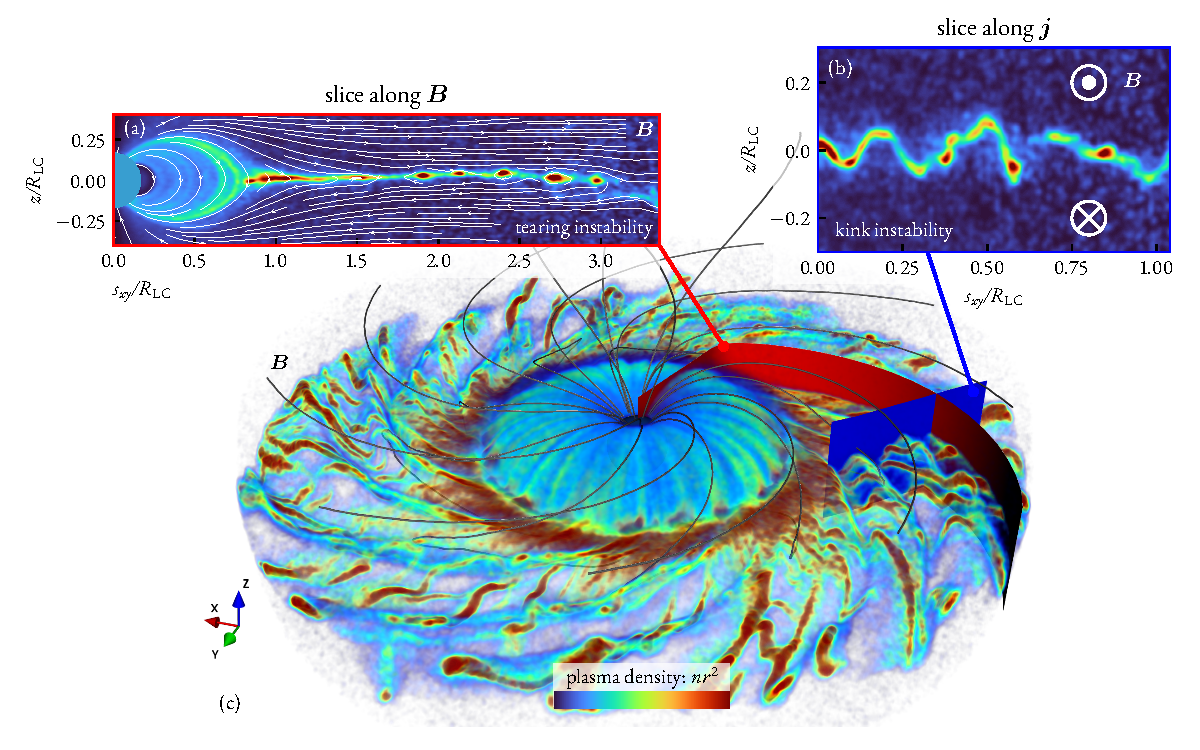
\includegraphics[width=\columnwidth,trim={10 10 10 5},clip]{figures/ch3-pulsar/fig3.pdf}
\caption{3D rendering of the plasma density (compensated by $r^2$) from a simulation of an aligned rotator (\texttt{R75\_ang0}). 3D rendering (panel c) is accompanied by the two slices (a and b, also visible in 3D as red and blue planes). One of the slices (a) is along the upstream magnetic field, while the second one (b) is along the direction of the current perpendicular to the magnetic field. Overdense elongated tubes in panel (c) are the 3D flux ropes, the plasmoids, which are produced as a result of the non-linear tearing instability. In a 2D slice (a) the dynamics of both the current sheet and the plasmoids themselves look very similar to those in localized current sheet simulations. In panel (b) kink instability is visible, which deforms the current sheet in the direction perpendicular to the direction of the tearing instability. An animated version of this plot is available with the following link: \url{https://youtu.be/-YXJ4yTlhWw}.}
\label{fig:psr-pulsar3d}
\end{figure}

In the rotating frame the dynamics of the reconnecting current sheet in slice \ref{fig:psr-pulsar3d}a is very similar to the one in a 2D Harris sheet, except for the fact that both the upstream and the current sheet are flying outwards with bulk $\Gamma\sim \mathcal{O}(1)$. In the upstream (above and below the current sheet) the plasma motion is strictly constrained by magnetic field lines. Cold plasma and opposing magnetic field lines are brought together by an $\left(\bm{E}\times\bm{B}\right)_z$ drift (shown in Figure~\ref{fig:psr-reconnection}a); the current sheet then becomes unstable and tears producing plasmoids (shown with magenta contours). The dimensionless rate of inflow is set by reconnection; this value can be directly measured for an axisymmetric pulsar (Figure~\ref{fig:psr-reconnection}a). For our simulations this value is close to
\begin{equation}
    \beta_{\rm rec} \equiv \frac{\left(\bm{E}\times\bm{B}\right)_{\rm in}}{|\bm{B}|^2} \approx 0.1\text{-}0.2.
\end{equation}

\begin{figure}[htb]
    \sidebysidecaption{0.555\linewidth}{0.42\linewidth}{
        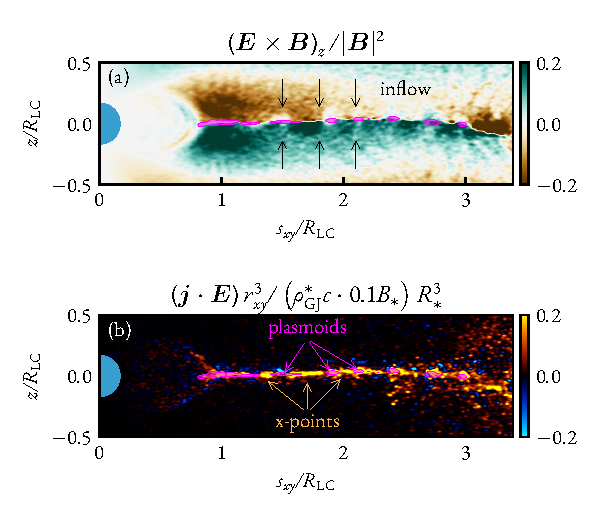
\includegraphics[width=\columnwidth,trim={10 10 10 5},clip]{figures/ch3-pulsar/fig4.pdf}
    }{
        \caption{Two panels show different quantities in the same slice as Figure~\ref{fig:psr-pulsar3d}a. (a) shows the  $\bm{E}\times\bm{B}$ inflow rate into the current sheet; this corresponds to the rate at which the reconnection of magnetic field lines occur, roughly, $\beta_{\rm rec}\sim 0.1$. In panel (b) we plot the work done by the electric field on current-carrying charges (compensated by $r_{xy}^3$). This term is responsible for the dissipation of the spin-down Poynting flux in the magnetosphere. The dissipation is mostly focused in the thin equatorial region, the current sheet. On both panels we overplot the plasmoids in magenta (they are clearly visible in Figure~\ref{fig:psr-pulsar3d}a).}
        \label{fig:psr-reconnection}
    }
\end{figure}

\subsection*{\small\it Magnetic energy dissipation via reconnection}

Reconnecting magnetic field in the current sheet generates an accelerating non-ideal electric field in the direction of the $\nabla\times \bm{B}$, same as the direction of the current in Figure~\ref{fig:psr-pulsarslice}a (in Figure~\ref{fig:psr-pulsar3d}a and Figure~\ref{fig:psr-reconnection}a,b that corresponds to the out-of-plane direction). Its magnitude is of the order of $E_{\rm rec}\sim \beta_{\rm rec}B_{\rm up}$, where $B_{\rm up}$ is the magnetic field strength in the upstream. Because of the emergence of $\bm{j}\cdot \bm{E}$ (shown in Figure~\ref{fig:psr-reconnection}b) the Poynting flux radiated by the star \eqref{eq:psr-edot} dissipates in the magnetosphere. As seen in Figure~\ref{fig:psr-reconnection}b dissipation occurs exclusively in the current sheet outside the light cylinder, where the energy of the electromagnetic field is converted into the kinetic energy of plasma through magnetic reconnection. According to Poynting's theorem:

\begin{equation}
\label{eq:psr-poynting-th}
    L(r) - L_0 \equiv \oiint\limits_{R_{\rm LC}}^r \bm{S} d\bm{a} = -\iiint \bm{j}\cdot \bm{E}d^3\bm{r}.
\end{equation}
\noindent This yields to the fact that $L(r)$ is a decaying function of radius. Figure~\ref{fig:psr-dissipation} shows the $L(r)$ from one of our simulations with $\chi=0^\circ$ computed using the flux of the Poynting vector (blue line), and the volume integral of $\bm{j}\cdot\bm{E}$ (red line). Orange band corresponds to an analytical model described in the next paragraph.

To understand the dependence of $L(r)$ it is useful to build a simple analytical model of the Poynting flux dissipation in the current sheet. For $\chi=90^\circ$ rotator this model has been studied by \cite{2020A&A...642A.204C}; here we focus on $\chi=0^\circ$. As mentioned earlier, the dissipation of Poynting flux is caused by the work done by the reconnection electric field, $\bm{j}\cdot\bm{E}$, as described by \eqref{eq:psr-poynting-th}. The strength of the electric field generated due to magnetic reconnection at a given distance $r$ from the star is $E_{\rm rec}(r)\sim\beta_{\rm rec} B_{\rm up}(r)$. Here the reconnecting magnetic field is a combination of poloidal and toroidal components from \eqref{eq:psr-bfields} $B_{\rm up}(r) =\sqrt{B_\runit^2 + B_\phiunit^2}$.\footnote{This is the main difference with the $\chi=90^\circ$ case, where only toroidal component of the magnetic field is reconnecting.} Since $(4\pi/c)\bm{j}=\nabla\times\bm{B}$, current, generated during the reconnection can be estimated as $j\sim c B_{\rm up} / (2\pi \delta_{\rm cs})$, where $\delta_{\rm cs}$ is the characteristic width of the current sheet. Thus, the volume integral in \eqref{eq:psr-poynting-th} reduces to:

\begin{equation}
\label{eq:psr-luminosity-int}
    L(r) - L_0 = -\int\limits_{R_{\rm LC}}^r dr\int\limits_0^{2\pi}d\phi \int\limits_0^\pi d\theta r^2\sin{\theta} \left(\frac{\beta_{\rm rec} c}{2\pi \delta_{\rm cs}}B_{\rm up}^2\right).
\end{equation}
\noindent Integral over the azimuthal angle $\phi$ is trivial because of the axisymmetry. Integral over the polar angle, $\theta$, at each $r$ is accumulated in a small region near the equator ($\theta=\pi/2$) of angular size $\Delta \theta\sim \delta_{\rm cs}/r$ (which is the current sheet highlighted in Figure~\ref{fig:psr-reconnection}b). Integrating \eqref{eq:psr-luminosity-int} using expressions for the fields from \eqref{eq:psr-bfields} then yields

\begin{equation}
\label{eq:psr-luminosity}
    \frac{L(r)}{L_0} = 1 - \beta_{\rm rec}\left(\ln{\frac{r}{R_{\rm LC}}}
    +\frac{1}{2}\left(1 -\left[\frac{r}{R_{\rm LC}}\right]^{-2}\right)\right).
\end{equation}

\noindent The logarithmic term in this relation corresponds to the dissipation of the toroidal field, $B_\phiunit$, while the second term corresponds to the dissipation of poloidal field, $B_{\runit}$. At large distances, $r\gg R_{\rm LC}$ the first term prevails, as the field is almost purely toroidal. However, for the short region, $R_{\rm LC}<r<2R_{\rm LC}$, considered in Figure~\ref{fig:psr-dissipation} contributions from both terms are important. Orange band in Figure~\ref{fig:psr-dissipation} corresponds to \eqref{eq:psr-luminosity} with $\beta_{\rm rec}$ varying from $0.09$ to $0.12$ (this number can be directly measured from Figure~\ref{fig:psr-reconnection}a). For other values of $\chi$ our results are consistent with earlier works (PIC: \citealt{2015ApJ...801L..19P}, and MHD: \citealt{2013MNRAS.435L...1T}). Namely, the spin-down luminosity near the light cylinder $\oint \bm{S}d\bm{a}\approx L_0(1 + \sin^2{\chi})$, and for larger values of $\chi$ we see inhibited dissipation in the current sheet, as the jump of the magnetic field across the current sheet is diminished for larger $\chi$.

\begin{figure}[htb]
    \sidebysidecaption{0.555\linewidth}{0.42\linewidth}{
        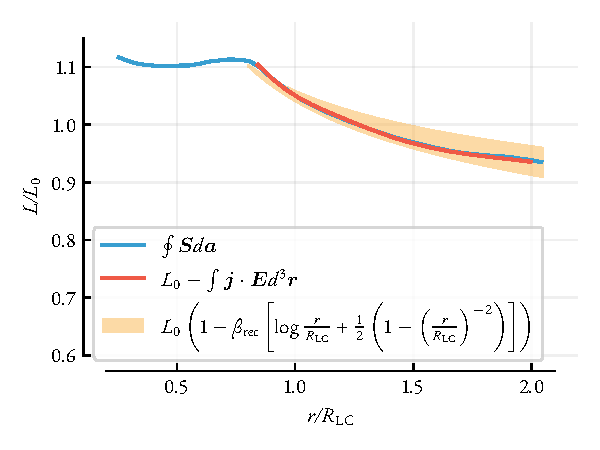
\includegraphics[width=\columnwidth,trim={10 10 10 5},clip]{figures/ch3-pulsar/fig5.pdf}
    }{
    \caption{Dissipation of the spin-down Poynting flux in the outer magnetosphere from a simulation of an aligned rotator. The blue line is the direct measurement of the Poynting flux vs $r$. The red line shows the work done by the electric field on charges, $\bm{j}\cdot\bm{E}$, which, according to Poynting's theorem, accounts for the dissipation of the Poynting flux. Orange band is the theoretical fit \eqref{eq:psr-luminosity} with $\beta_{\rm rec}\approx 0.09\textrm{-}0.12$. $L_0$ is computed from \eqref{eq:psr-edot}. A slight increase of $L$ with respect to $L_0$ in the inner magnetosphere is due to the fact that the Y-point in our simulation is slightly shifted inside w.r.t. the $r/R_{\rm LC} = 1$; this leads to slightly more open field lines and thus more Poynting flux.}
    \label{fig:psr-dissipation}
    }
\end{figure}

Dissipated energy of the magnetic field during the reconnection in the current sheet is deposited into plasma particles. In the next section we focus on particle energization in the current sheet and its consequences on the observed high-energy emission in $\gamma$-ray pulsars.

\section{Particle acceleration and $\gamma$-ray emission}
\label{sec:psr-radiation}
Relativistic magnetic reconnection is known to produce non-thermal particle population \citep{2014ApJ...783L..21S}; reconnection in the current sheets of neutron star magnetospheres is no exception. These energized particles are believed to radiate via synchrotron mechanism, producing the pulsed high-energy emission observed in $\gamma$-ray pulsars \citep{2016MNRAS.457.2401C,PSAS18}.

\subsection*{\small\it Efficiency of magnetic reconnection and synchrotron cooling}

Main parameter that determines the efficiency of particle acceleration during reconnection is \emph{the magnetization} of the upstream (unreconnected) plasma, $\sigma$. For the given background magnetic field, $B$, and the number density of inflowing plasma, $n$, this dimensionless parameter is equal to twice the ratio of the magnetic energy density and the rest mass energy density of plasma. Or equivalently, it is equal to the square of the ratio of gyrofrequency to plasma frequency (for cold particles with $\beta\gamma\approx 1$):
\begin{equation}
    \sigma \equiv \frac{B^2/4\pi}{n m_e c^2} = \left(\frac{\omega_{B}}{\omega_{{\rm p}e}}\right)^2.
\end{equation}
\noindent This parameter, which is $\gg 1$ in case of relativistic reconnection, determines the characteristic maximum energy to which particles can be accelerated in the single x-point (or x-line in 3D, see Figure~\ref{fig:psr-reconnection}b). If secondary reacceleration is prohibited, i.e. if particles leave the system as soon as they get accelerated in a single x-point, their non-thermal distribution function extends at most to energies of a few times $\sigma m_e c^2$. Energized particles, however, may either then reenter the current sheet or become trapped in plasmoids and get accelerated again via secondary processes to even higher energies \citep{2018MNRAS.481.5687P,2021ApJ...912...48H}. However, as we demonstrate below, in pulsar magnetospheres with realistic parameters this is almost impossible due to the chaotic nature of the current sheet and the synchrotron losses. 

Synchrotron cooling may slow down particles at timescales comparable to the acceleration timescale in the current sheet, affecting the emerging non-thermal particle distribution. The efficiency of cooling is determined by the strength of the magnetic field. This can be conveniently quantified with a dimensionless number, $\gamma_{\rm rad}$, easily transferable to PIC simulations. This number corresponds to the Lorentz factor of particles for which the synchrotron cooling timescale in a given background magnetic field $B$ is comparable to the acceleration timescale due to reconnection (acceleration in an electric field of strength $E\sim \beta_{\rm rec}B$):

\begin{equation}
    |e|\beta_{\rm rec}B c = \frac{2}{3}r_e^2 c B^2 \gamma_{\rm rad}^2,
\end{equation}
\noindent where $r_e=e^2/m_e c^2$ is the classical radius of the electron.\footnote{In terms of PIC simulations, defining dimensionless $\gamma_{\rm rad}$ is equivalent to upscaling the classical electron radius, $r_e$, which would otherwise be severely underresolved. Also note, that in this rough definition the magnetic field is considered to be exactly perpendicular to the motion of a particle. In our simulations, as well as in reality, particles flying at small pitch angles w.r.t. the magnetic field will be cooled less efficiently. Thus, $\gamma_{\rm rad}$ can be thought of as just a proxy for the average cooling efficiency for a population of isotropically distributed particles.} Particles with $\gamma \gg \gamma_{\rm rad}$ will lose their energies as soon as they are exposed to a perpendicular magnetic field component much faster than they are able to accelerate, while the opposite is true for particles with $\gamma \ll \gamma_{\rm rad}$. 

Guided by the $\sigma$-limit of the acceleration during magnetic reconnection, we will call the cooling \emph{strong} when $\gamma_{\rm rad} < \sigma$, while the opposite case will be referred to as the \emph{weak cooling} regime. Naively, one could think that in the reconnection process with strong cooling particles cannot gain energies higher than $\gamma_{\rm rad} m_e c^2$, as for these particles the cooling becomes faster than the acceleration. However, this is not necessarily true, as the acceleration takes place in the region of the current sheet where there is virtually no cooling (the magnetic field is zero in the x-points; we show this below, and this has also been demonstrated in 2D simulations by \citealt{2019ApJ...877...53H}). On the other hand, in the strong cooling regime once particles leave the accelerating regions (either back to the upstream or into plasmoids), they very quickly lose their energies without a chance to get reaccelerated again to energies larger than a few $\sigma m_e c^2$. This results in qualitatively different radiation spectra in two different cooling regimes. While cutoff energies of photons are still comparable, as plasma particles are still able to accelerate to $\gamma\sim \sigma$ in x-points, the peak of the radiation is shifted to lower energies in the strong cooling regime ($\gamma_{\rm rad}/\sigma \ll 1$), because particles are unable to retain energies $\gamma>\gamma_{\rm rad}$ for longer times.

The value of $\gamma_{\rm rad}$ (close to the light cylinder) only depends on the magnetic field strength:
\begin{equation}
    \gamma_{\rm rad}^{\rm LC}\approx 10^5\left(\frac{B_{\rm LC}}{10^5~\text{G}}\right)^{-1/2},
\end{equation}
\noindent which we know rather reliably for pulsars by extrapolating the magnetic field strength at the surface. The magnetization, $\sigma_{\rm LC}$, on the other hand, depends on plasma density near the light cylinder which is generally unknown. However, we can estimate that approximately, by assuming that the cutoff frequency of the $\gamma$-ray photons corresponds to the synchrotron peak energy for the highest-energy particles with $E\sim 10 \sigma_{\rm LC} m_e c^2$:
\begin{equation}
    \hbar \omega_B^{\rm LC} (10\sigma_{\rm LC})^2 \approx E_{\rm cut}.
\end{equation}
\noindent This provides a rough empirical estimate for $\sigma_{\rm LC}$. For the population of young pulsars $\sigma$ value is between $10^5$ and $10^6$, and the ratio $\gamma_{\rm rad}^{\rm LC}/\sigma_{\rm LC}$ varies between $0.5\text{-}2$ (for the Crab the value is $2$). We also note that the pulsars with stronger synchrotron cooling at the light cylinder typically have $\gamma$-ray spectra shifted to lower energies ($<0.1$ MeV).

In our simulations we keep $\sigma\gg 1$ in the outer magnetosphere (to ensure the reconnection is in the ultra-relativistic regime), and vary the ratio $\gamma_{\rm rad}/\sigma$. Following the discussion earlier, this ratio determines the relative importance of the effects of synchrotron cooling on reconnection dynamics, and, as we demonstrate later, results in qualitatively different high-energy radiation spectra.

\subsection*{\small\it Particle distributions and photon spectra in the radiatively cooled magnetosphere}

For the simulation \texttt{R75\_ang0} magnetization parameter in the upstream, shown in Figure~\ref{fig:psr-sigma}, is close to $\sigma_{\rm LC}\sim 10^3$ in the upstream (as shown with the linear plot on the right) and drops to zero inside the current sheet, where the magnetic field reconnects. This means that the characteristic energies to which particles can get accelerated in the current sheet is comparable to $\sigma m_e c^2$ (as will be demonstrated shortly).

\begin{figure}[htb]
    \sidebysidecaption{0.555\linewidth}{0.42\linewidth}{

        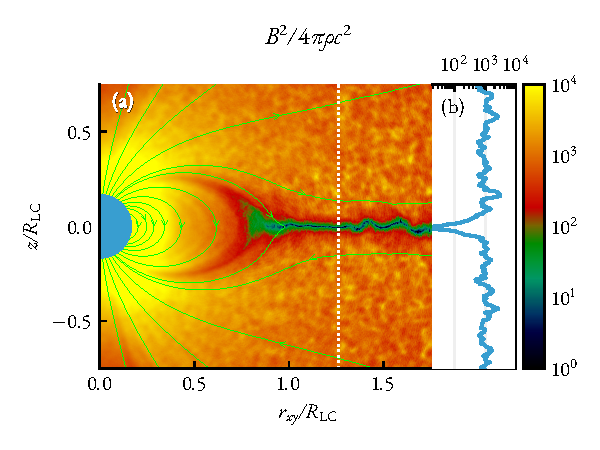
\includegraphics[width=\columnwidth,trim={10 10 10 5},clip]{figures/ch3-pulsar/fig6.pdf}
    }{
        \caption{(a): plasma magnetization parameter, $\sigma$, in a poloidal slice of the simulation \texttt{R75\_ang0}. 1D slice of the $\sigma$ across the current sheet is shown in panel (b). Magnetization of the upstream is close to $10^3$, while the background plasma density $n\sim \text{few}\cdot n_{\rm GJ}^*(R_*/r)^2$. Magnetic field lines are shown with green in panel (a).}
        \label{fig:psr-sigma}
    }
\end{figure}

Let us consider distribution functions for $e^\pm$ in different regions of our simulation \texttt{R75\_ang0}, as shown in Figure~\ref{fig:psr-spatial_spectra}. On a poloidal slice in panel \ref{fig:psr-spatial_spectra}a we show the bulk Lorentz factor of the plasma, $\Gamma = \sqrt{1 + \bm{U}^2/c^2}$, which is computed using the bulk four-velocity, $\bm{U} = \int \bm{u}f(\bm{u})d^3\bm{r}$. Panels \ref{fig:psr-spatial_spectra}b, \ref{fig:psr-spatial_spectra}c, and \ref{fig:psr-spatial_spectra}d show distribution functions of the electrons and positrons in three different regions: in the separatrix (last closed field line), in the current sheet, and in the upstream correspondingly. \emph{Upstream} plasma is relatively cold; electrons and positron are carried outwards almost radially via an $\bm{E}\times\bm{B}$ drift, gaining characteristic bulk Lorentz factors of $\Gamma \sim 10$ on scales of our simulation (Figure~\ref{fig:psr-spatial_spectra}d). On \emph{the separatrix} (Figure~\ref{fig:psr-spatial_spectra}b) both electrons and positrons from the surface are marginally accelerated by an unscreened electric field, gaining energies close to $\langle\gamma \rangle\sim 10\text{-}100$. This region also hosts hot electrons returning from the current layer, which is evident from the excess of electrons at Lorentz factors of a few $10^2$ shown in Figure~\ref{fig:psr-spatial_spectra}b. 

These two regions, the upstream and the separatrix, act as an ``intake'' and an ``exhaust'' for \emph{the current sheet}. It is important to note, that particles in these regions are generally exposed to a substantial orthogonal magnetic field component. This means that high-energy particles from the current sheet cannot exist there for timescales longer than the short cooling time. Thus, the main role in shaping the observed $\gamma$-ray emission is played by the current sheet, where constant release of magnetic energy sustainably accelerates particles in x-lines, where the magnetic field strength is zero (the cooling is non-existent).

In the current sheet (Figure~\ref{fig:psr-spatial_spectra}c) we see a substantial non-thermal particle population, extending to $\gamma\sim \sigma\sim 500\text{-}1000$. The bulk motion of the current sheet, on the other hand, has a Lorentz factor of $\Gamma\sim 10\text{-}100$, consistent with characteristic velocities of relativistic flows along the current sheet during the reconnection, $\Gamma\sim \sqrt{\sigma}$.\footnote{Slight enhancement is due to the fact that there is a bulk $\bm{E}\times\bm{B}$ outflow of the current sheet, similar to the wind in the upstream.} Notice also, that the distributions of electrons and positrons are slightly different: positrons extend to slightly higher energies. This is due to the fact that the electric field generated during reconnection ``pushes'' the electrons opposite to the global $\bm{E}\times\bm{B}$ drift, which is charge-invariant and directed radially outward (in Figure~\ref{fig:psr-pulsar3d}a the reconnection electric field is pointing in the out-of-plane direction). This difference in the electrons and positrons has been observed in earlier simulations \citep[see, e.g.,][]{PSAS18}; however, it almost vanishes for large obliquity angles, $\chi$, which we also see in our simulations.

\begin{figure}[htb]
\centering
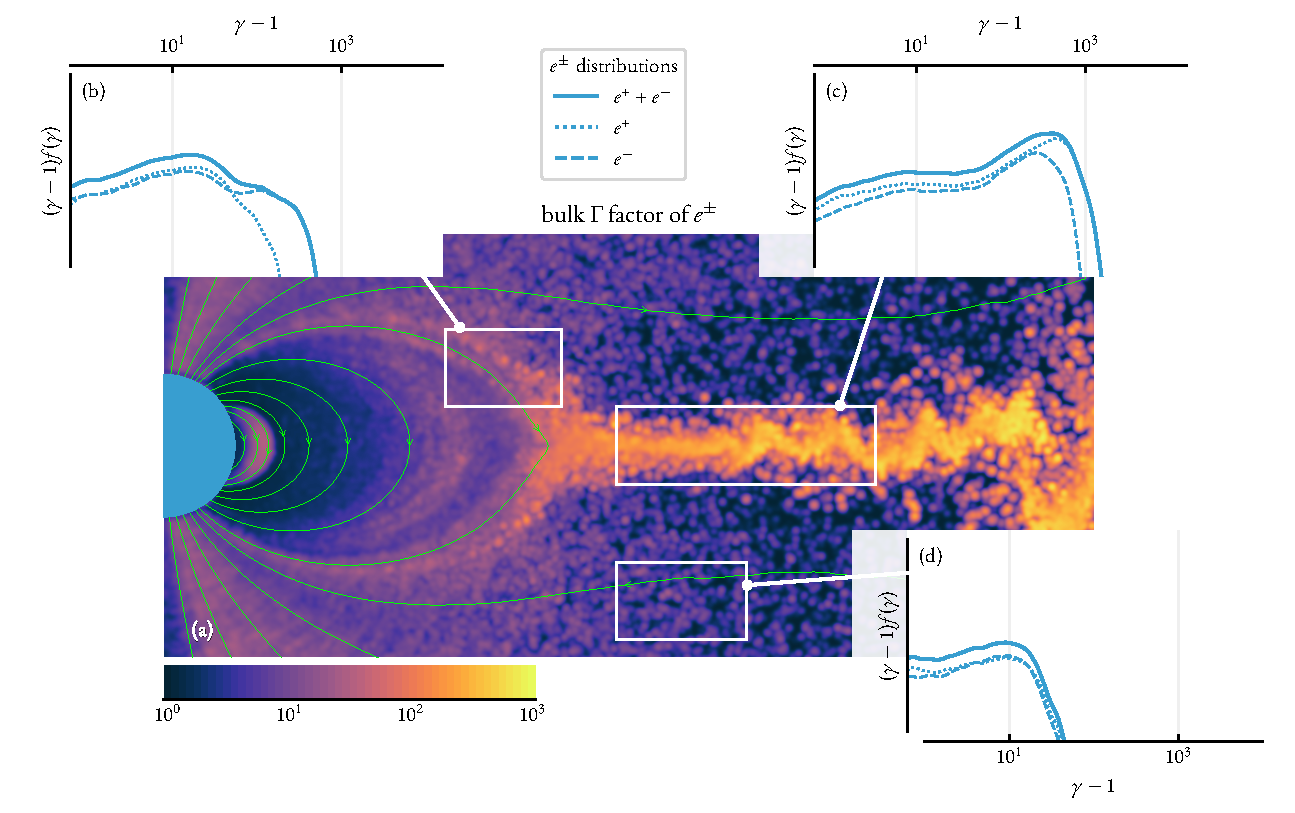
\includegraphics[width=\columnwidth,trim={10 0 10 5},clip]{figures/ch3-pulsar/fig7.pdf}
\caption{Distribution functions of electrons and positrons measured in different locations of our simulation. Bulk Lorentz factor is shown in panel (a). Panels (b), (c), and (d) show distribution functions in the separatrix, the current layer and the upstream, correspondingly. Plasma in the upstream is typically cold with a bulk outflow Lorentz factor of a few. As expected, the highest energy particles are produced in the current layer where magnetic reconnection occurs.}
\label{fig:psr-spatial_spectra}
\end{figure}

We now study the effects of different cooling regimes, i.e., different values of $\gamma_{\rm rad}/\sigma$, on both the global kinetic solution, as well as the particle and the photon spectra. Since an aligned pulsar with $\chi=0^\circ$ is pathological as it does not produce any modulated emission, most of the $\gamma$-ray pulsars are thought to have inclination angles $0<\chi<90^\circ$. We thus closely inspect two simulation setups with $\chi=20^\circ$ and $\chi=60^\circ$ (these simulations will be referred to as \texttt{R75\_ang20}, and \texttt{R75\_ang60}; all the other parameters except for the inclination angle are the same as in \texttt{R75\_ang0}). In a series of runs we keep $\sigma_{\rm LC}\approx 500\text{-}1000$ and vary $\gamma_{\rm rad}^{\rm LC}$ to capture the following regimes: $\gamma_{\rm rad}^{\rm LC}/\sigma_{\rm LC}=1/15,~1/3,~2,\infty$ (where $\gamma_{\rm rad}=\infty$ corresponds to simulation without synchrotron cooling; for a future reference, these simulations we denote as \texttt{R75\_ang20\_gr1o15}, \texttt{R75\_ang60\_gr1o15}, ..., \texttt{R75\_ang60\_grINF}).

\begin{figure}[htb]
    \sidebysidecaption{0.555\linewidth}{0.42\linewidth}{
        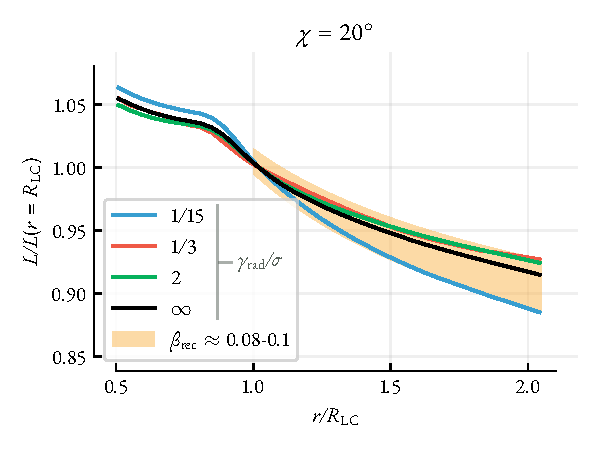
\includegraphics[width=\columnwidth,trim={10 0 10 5},clip]{figures/ch3-pulsar/fig10.pdf}
    }{
        \caption{Poynting flux dissipation as a function radius, $L(r)$, for different cooling regimes in \texttt{R75\_ang20}. Reconnection rate and, thus, the dissipation is only marginally affected by the strength of synchrotron cooling.}
        \label{fig:psr-rad-dissipation}
    }
\end{figure}

We find that the general structure of the current sheet is largely unaffected by the strength of synchrotron cooling. In the most extreme case $\gamma_{\rm rad}^{\rm LC}/\sigma_{\rm LC}=1/15$ plasmoids become slightly more compressed as radiation reaction suppresses the perpendicular plasma pressure which holds plasmoids in equilibrium counteracting the $\bm{j}\times\bm{B}$ force. Nevertheless, the rate of magnetic reconnection and, as a result, the Poynting-flux dissipation curves, $L(r)$, are only marginally affected as seen in Figure~\ref{fig:psr-rad-dissipation} for $\chi=20^\circ$. 

Particle distribution functions in the current sheet are also very similar in all of the cooling regimes, as shown in Figures~\ref{fig:psr-spec20}a and \ref{fig:psr-spec60}a. In all of the studied cases particles in the current are able to accelerate to $\sim\sigma_{\rm LC}$ in x-points, forming a power law of $f\propto \gamma^{-1}$ (for $\chi=60^\circ$ the spectrum is slightly steeper). Only in the most strongly cooled simulation we see that the cutoff of particle distribution is slightly shifted towards lower energies. This is most likely an effect of comparably small scale separation in our simulations, which will most likely be unnoticable for realistic systems. Since x-lines in 3D have finite extent, in a single encounter particles are unable to tap the full potential drop across it. Thus, typically, particles will need several encounters to be accelerated to highest energies. In the strongest cooling case, however, as soon as particles leave the x-point, they are cooled almost instantly either in the upstream or in plasmoids. These conclusions are consistent with 2D local simulations of radiative magnetic reconnection by \cite{2019ApJ...877...53H}. In weakly cooled simulations above $\gamma>\sigma_{\rm LC}$ we see a smooth transition to $\gamma^{-2.5}\text{-}\gamma^{-3}$ and, eventually, to an almost exponential cutoff. We speculate that this transition, almost absent in simulations with strong cooling, might be indicative that particles are also experiencing brief secondary acceleration inside the compressing plasmoids as described by \cite{2018MNRAS.481.5687P,2021ApJ...912...48H}.

In Figures \ref{fig:psr-spec20}b and \ref{fig:psr-spec60}b we show spectra of the emitted synchrotron photons for both $\chi=20^\circ$ and $\chi=60^\circ$ simulations at different cooling regimes. In all cases we see a recurring pattern in photon spectra: a rise $\nu F_\nu\propto \nu$, a transition with a peak and a decay at higher energies. Power-law index for the distribution of photons is roughly consistent with the power-law index for the distribution of particles, i.e., $f\propto \gamma^{-p}$ leads to $\nu F_\nu \propto \nu^{-(p-3)/2}$. We see a shift of the emission peak towards lower energies for simulations with stronger cooling. Also note, that we do not observe significant intermittency at higher energies for the strong cooling simulation as predicted by \cite{2019ApJ...877...53H}. This is most likely due to a much worse scale separation, and the overall complexity in the structure of the current sheet, as compared to 2D simulations (in 2D this high energy intermittency was primarily caused by plasmoid merger events).

\begin{figure}[htb]
\centering
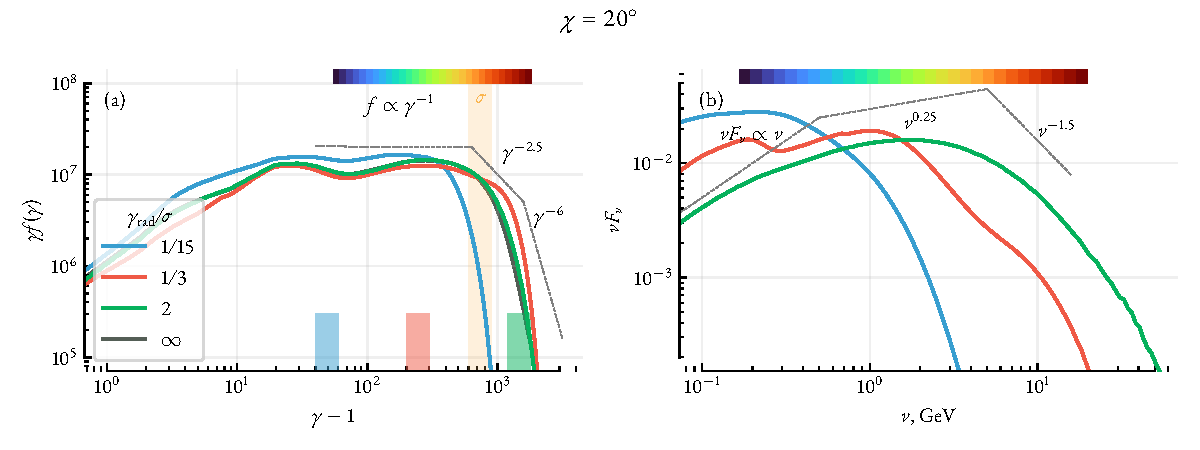
\includegraphics[width=\columnwidth,trim={10 0 10 5},clip]{figures/ch3-pulsar/fig9_a.pdf}
\caption{(a) particle and (b) photon spectra for the \texttt{R75\_ang20} simulation in different synchrotron cooling regimes. Effective $\sigma$ at the light cylinder is marked with a yellow stripe. Three smaller bars indicate the effective $\gamma_{\rm rad}$. Three power-law fits of $f\propto \gamma^{-p}$ in panel (a) translate to power-laws in photon spectra $\nu F_\nu \propto \nu^{-(p-3)/2}$. Colorbar at the top of both panels puts particle energies into correspondence with synchrotron peak energies, $\nu \propto \gamma^2 B_{\rm LC}$. While particle spectra look almost identical (except for the strongest cooled case), peaks of photons are shifted to smaller energies for smaller $\gamma_{\rm rad}/\sigma$. Only particles in the current layer are accounted for.}
\label{fig:psr-spec20}
\end{figure}

\begin{figure}[htb]
\centering
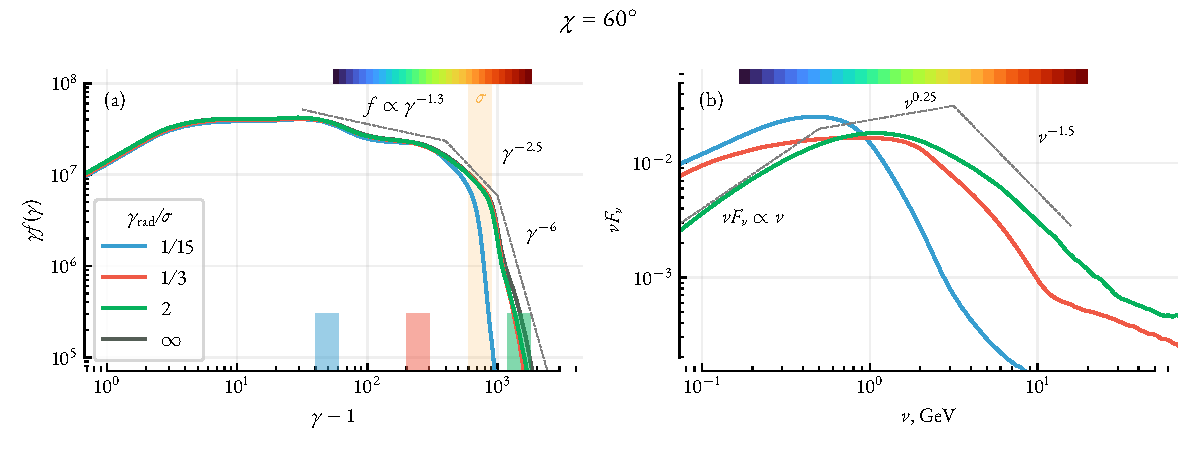
\includegraphics[width=\columnwidth,trim={10 0 10 5},clip]{figures/ch3-pulsar/fig9_b.pdf}
\caption{Same as in Figure~\ref{fig:psr-spec20} but for simulation \texttt{R75\_ang60}. Particle distributions are still largely unaffected by cooling, while the peaks of photon spectra are shifted towards lower energies for stronger cooling simulations.}
\label{fig:psr-spec60}
\end{figure}

\section{Discussion \& summary}

In this work we demonstrated the result from 3D PIC simulations of the neutron star magnetospheres with the synchrotron radiation reaction force included. Our primary focus was the energy dissipation and the plasma dynamics in the reconnecting current sheet. To be able to properly capture the kinetic physics, governing the energy extraction in the current layer we push the separation of macro-to-micro scales in our simulations to $\sim 200$, which allows to self-consistently model the hierarchical chain of plasmoids in the saturated tearing unstable regime. 

We show that the rate of inflow to reconnecting current sheet, which is controlled by plasma-kinetics at scales of microscopic x-lines, determines the dissipation rate in the entire magnetosphere. This puts a stringent constraint on how much energy can be dissipated in the current layer (and, ultimately, radiated) within a few light cylinders. From simulations we find that this dissipation rate is almost insensitive to both the bulk motion of the background unreconnected plasma, and the radiation efficiency.

We confirm that the particle distribution is almost unaffected by synchrotron cooling, with particles in the current sheet forming a hard power-law spectrum with steep cutoff at energies of $\sim \sigma_{\rm LC}m_e c^2$. Photon spectra, on the other hand, are largely different, with the stronger cooling simulations resulting in peaks shifted towards lower energies. 

These results are partly consistent with the observations by \emph{Fermi} satellite. However, we note an important difference: observations show that the pulsars with $\gamma$-ray peaks at lower energies have typically wider spectra resulting in almost constant value for the cutoff energy, $E_{\rm cut}$. This has also been confirmed in 2D localized simulations \citep{2019ApJ...877...53H}, where a wide spectrum with a slow $\nu F_\nu\propto \nu^{-1/2}$ decay was observed for the cases with strongest synchrotron cooling. This high-energy tail was mostly accumulated in the intermittent events of large plasmoid mergers, abundant in 2D simulations. In our 3D simulations, however, the limited scale separation does not allow to capture many of these events.